\documentclass{beamer}
\usetheme{Boadilla}
\usepackage[utf8]{inputenc}
\usepackage[fixlanguage]{babelbib}
\usepackage[spanish,mexico]{babel}
\usepackage{color,soul}
\usepackage{graphicx}
\usepackage{caption}
\usepackage{tikz}
\usepackage{tikz-uml}
\usetikzlibrary{arrows.meta,
                matrix,
                positioning,
                automata, 
                decorations.pathreplacing
                }
\usepackage{skak}
\usepackage{tikz}
\usepackage{advdate}
\usetikzlibrary{shapes.arrows}
\tikzset{
    myarrow/.style={
        draw,
        fill=orange,
        single arrow,
        minimum height=3.5ex,
        single arrow head extend=1ex
    }
}
\newcommand{\arrowup}{%
\tikz [baseline=-0.5ex]{\node [myarrow,rotate=90] {};}
}
\newcommand{\arrowdown}{%
\tikz [baseline=-1ex]{\node [myarrow,rotate=-90] {};}
}
\definecolor{rojo}{RGB}{255,0,0}
\definecolor{verde}{RGB}{0,255,0}
\definecolor{azul}{RGB}{0,0,255}
\definecolor{naranja}{RGB}{255,69,0}
\definecolor{dorado}{RGB}{255,125,0}
\definecolor{morado}{RGB}{128,0,128}
\definecolor{acian}{RGB}{0,255,255}
\definecolor{misol}{RGB}{255,255,0}
\definecolor{minegro}{RGB}{0,0,0}
\definecolor{mimorado}{RGB}{241,101,244}
\usetikzlibrary{matrix}
\makeatletter
\newcounter{qrr@tikz@omino}
\newcounter{qrr@tikz@omino@up}
\newcounter{qrr@tikz@omino@right}
\tikzset{
    omino/.style={/tikz/omino/.cd,#1},
    omino/distance/.initial=1,
    omino/radius/.initial=.5,
    omino/at/.style={/tikz/shift={(#1)}},
    omino/rotate/.style={/tikz/rotate=#1},
    omino/s/.code=
        \setcounter{qrr@tikz@omino}{0}%
        \setcounter{qrr@tikz@omino@up}{0}%
        \setcounter{qrr@tikz@omino@right}{0}%
        \pgfkeysalso{/tikz/insert path={(0,0) node[/tikz/omino/nodes/.try,/tikz/omino/node normal/.try,/tikz/omino/node start/.try] {\qrr@tikz@omino@text@start}}},
    omino/u/.code=%
        \stepcounter{qrr@tikz@omino}%
        \stepcounter{qrr@tikz@omino@up}%
        \pgfkeysalso{/tikz/insert path={
            to[/tikz/omino/how] ++(up:#1)
            node[/tikz/omino/nodes/.try,/tikz/omino/node normal/.try,/tikz/omino/node up/.try]{\qrr@tikz@omino@text@up}}},
    omino/d/.code=%
        \stepcounter{qrr@tikz@omino}%
        \addtocounter{qrr@tikz@omino@up}{-1}%
        \pgfkeysalso{/tikz/insert path={
            to[/tikz/omino/how] ++(down:#1)
            node[/tikz/omino/nodes/.try,/tikz/omino/node normal/.try,/tikz/omino/node down/.try]{\qrr@tikz@omino@text@down}}},
    omino/l/.code=%
        \stepcounter{qrr@tikz@omino}%
        \addtocounter{qrr@tikz@omino@right}{-1}%
        \pgfkeysalso{/tikz/insert path={
            to[/tikz/omino/how] ++(left:#1)
            node[/tikz/omino/nodes/.try,/tikz/omino/node normal/.try,/tikz/omino/node left/.try]{\qrr@tikz@omino@text@left}}},
    omino/r/.code=%
        \stepcounter{qrr@tikz@omino}%
        \stepcounter{qrr@tikz@omino@right}%
        \pgfkeysalso{/tikz/insert path={
            to[/tikz/omino/how] ++(right:#1)
            node[/tikz/omino/nodes/.try,/tikz/omino/node normal/.try,/tikz/omino/node right/.try] {\qrr@tikz@omino@text@right}}},
    omino/u/.default=\pgfkeysvalueof{/tikz/omino/distance},
    omino/d/.default=\pgfkeysvalueof{/tikz/omino/distance},
    omino/l/.default=\pgfkeysvalueof{/tikz/omino/distance},
    omino/r/.default=\pgfkeysvalueof{/tikz/omino/distance},
    omino/how/.style=,
    omino/reset/.code=
        \pgfutil@in@_{#1}%
        \ifpgfutil@in@
            \qrr@tikz@omino@split#1\relax
        \else
            \edef\pgf@tempa{\csname qrr@tikz@omino@coords@#1\endcsname}%
            \expandafter\qrr@tikz@omino@split\pgf@tempa\relax
        \fi
        \pgfkeysalso{/tikz/insert path={(omino-n-#1.center) node[/tikz/omino/nodes/.try, /tikz/omino/node reset/.try] {\qrr@tikz@omino@text@reset}}},
    omino/do/.code={\@tfor\@next:=#1\do{\pgfkeysalso{/tikz/omino/\@next}}},
    omino/node reset/.style={draw=none,fill=none},
    omino/node normal/.style={
        name=omino-n-\number\c@qrr@tikz@omino,
        alias=omino-n-\number\c@qrr@tikz@omino@right_\number\c@qrr@tikz@omino@up,
        omino/@store coords
    },
    omino/@store coords/.code=
        \expandafter\xdef\csname qrr@tikz@omino@coords@\arabic{qrr@tikz@omino}\endcsname
        {\number\c@qrr@tikz@omino@right_\number\c@qrr@tikz@omino@up},
    omino/Text/.code 2 args=\expandafter\edef\csname qrr@tikz@omino@text@#1\endcsname{#2},
    omino/Text={up}{},omino/Text={down}{},omino/Text={left}{},omino/Text={right}{},omino/Text={start}{},omino/Text={reset}{}
}
\def\qrr@tikz@omino@split#1_#2\relax{\setcounter{qrr@tikz@omino@right}{#1}\setcounter{qrr@tikz@omino@up}{#2}}

\tikzset{
    omino/x mirror/.style={/tikz/cm={-1,0,0,1,(0,0)}},
    omino/y mirror/.style={/tikz/cm={1,0,0,-1,(0,0)}}
}

\tikzset{fun/.code={\pgfmathtruncatemacro\@fun{\number\c@qrr@tikz@omino/4*100}\pgfkeysalso{fill=blue!\@fun!red}}}
\makeatother
\tikzset{
    tetris/.style={/tikz/tetris/.cd,#1},
    tetris/1/.style={/tikz/omino={do=suuu}},
    tetris/2/.style={/tikz/omino={do=suur}},
    tetris/6/.style={/tikz/omino={do=suul}},
    tetris/3/.style={/tikz/omino={do=suru}},
    tetris/7/.style={/tikz/omino={do=sulu}},
    tetris/4/.style={/tikz/omino={do=surd}},
    tetris/8/.style={/tikz/omino={do=s}},
    tetris/9/.style={/tikz/omino={do=s}},
    tetris/0/.style={/tikz/omino={do=s}},
    tetris/5/.style={/tikz/omino={s,u,u,reset=1,r}}
}
\makeatletter

\makeatother
\newcommand*{\thesamepictureeverywhere}{\matrix[column sep=.5cm, row sep=.5cm, ampersand replacement=\&] {
\path [tetris=1];  \&
\path [tetris=6]; \& 
\path [tetris=2]; \&
\path [tetris=3];  \& 
\path [tetris=7]; \&
\path [tetris=4];  \&
\path [tetris=8]; \&
\path [tetris=9];  \&
\path [tetris=0];  \&
\path [tetris=5];\\};}

\tikzset{
    tetris/1/.prefix style={/tikz/omino/nodes/.append style={fill=rojo,text=white}},
    tetris/2/.prefix style={/tikz/omino/nodes/.append style={fill=azul}},
    tetris/6/.prefix style={/tikz/omino/nodes/.append style={fill=acian}},
    tetris/3/.prefix style={/tikz/omino/nodes/.append style={fill=verde}},
    tetris/7/.prefix style={/tikz/omino/nodes/.append style={fill=dorado}},
    tetris/4/.prefix style={/tikz/omino/nodes/.append style={fill=naranja}},
    tetris/8/.prefix style={/tikz/omino/nodes/.append style={fill=misol}},
    tetris/9/.prefix style={/tikz/omino/nodes/.append style={fill=mimorado}},
    tetris/0/.prefix style={/tikz/omino/nodes/.append style={fill=minegro}},
    tetris/5/.prefix style={/tikz/omino/nodes/.append style={fill=morado}},
    omino/Text={start}{.}
}
%% Algoritmo siempre termina 
% en la 6, Alfgoritmo siempre termina y la definicion esta en ingles. 
% Grarantia de resultados lleva punto.
% no. 
% en heuristica la condicion de terminacion es mas ambigua.


\setul{0.5ex}{0.3ex}
\setulcolor{blue}
\usepackage{scalerel,stackengine}
\def\buthickness{1pt}
\def\budefaultcolor{black}
\makeatletter
\newcommand\bunderline[1][\budefaultcolor]{\def\bucolor{#1}\bunderlineaux}
\newcommand\bunderlineaux[2][\buthickness]{%
  \ThisStyle{%
  \ifmmode%
    \setbox0=\hbox{\m@th$\SavedStyle#2$}
    \stackunder[2pt]{\copy0}{\textcolor{\bucolor}{\rule{\wd0}{#1}}}%
  \else%
    \xdef\butmpthickness{#1}%
    \prebunderlinewords#2 \endarg%
  \fi%
}}
\def\prebunderlinewords#1 #2\endarg{%
  \ifx\endarg#2\endarg\def\wdaugment{0pt}\else\def\wdaugment{.8ex}\fi%
  \bunderlinewords#1 #2\endarg%
}
\def\bunderlinewords#1 #2\endarg{%
    \setbox0=\hbox{#1\strut}%
    \stackengine{0pt}{\copy0}{\textcolor{\bucolor}{%
      \smash{\rule{\dimexpr\wd0+\wdaugment\relax}{\butmpthickness}}}}{U}{c}{F}{T}{S}% 
    \ifx\endarg#2\endarg\def\next{}\else\ \def\next{\bunderlinewords#2\endarg}\fi\next%
}
\newcommand\buonslide[1][black]{\def\butmpcolor{#1}\buonslideauxA}
\newcommand\buonslideauxA[1][\buthickness]{\def\butmpthickness{#1}\buonslideauxB}
\def\buonslideauxB<#1>#2{\onslide<#1>{%
  \rlap{\bunderline[\butmpcolor][\butmpthickness]{\phantom{#2}}}}#2}
\makeatother
\useinnertheme{default}
\beamertemplatenavigationsymbolsempty


\title[ABC implementado en Tetris]{Una implementación de la heurística Colonia de Abejas
Artificiales a una instancia del problema de la 3-Partición: 
Tetris}
\author{José Ricardo Rodríguez Abreu}
\institute[UNAM]{Universidad Nacional Autónoma de México}
\date{\AdvanceDate[+1]\today}

\begin{document}
 
\begin{frame}
\titlepage
\end{frame}

\section{Capítulo 1}
\subsection{Introducción al trabajo}
 
\begin{frame}
\frametitle{Tetris}

Tetris es uno de los videojuegos más conocidos con más de 170 millones de copias vendidas.

\begin{figure}
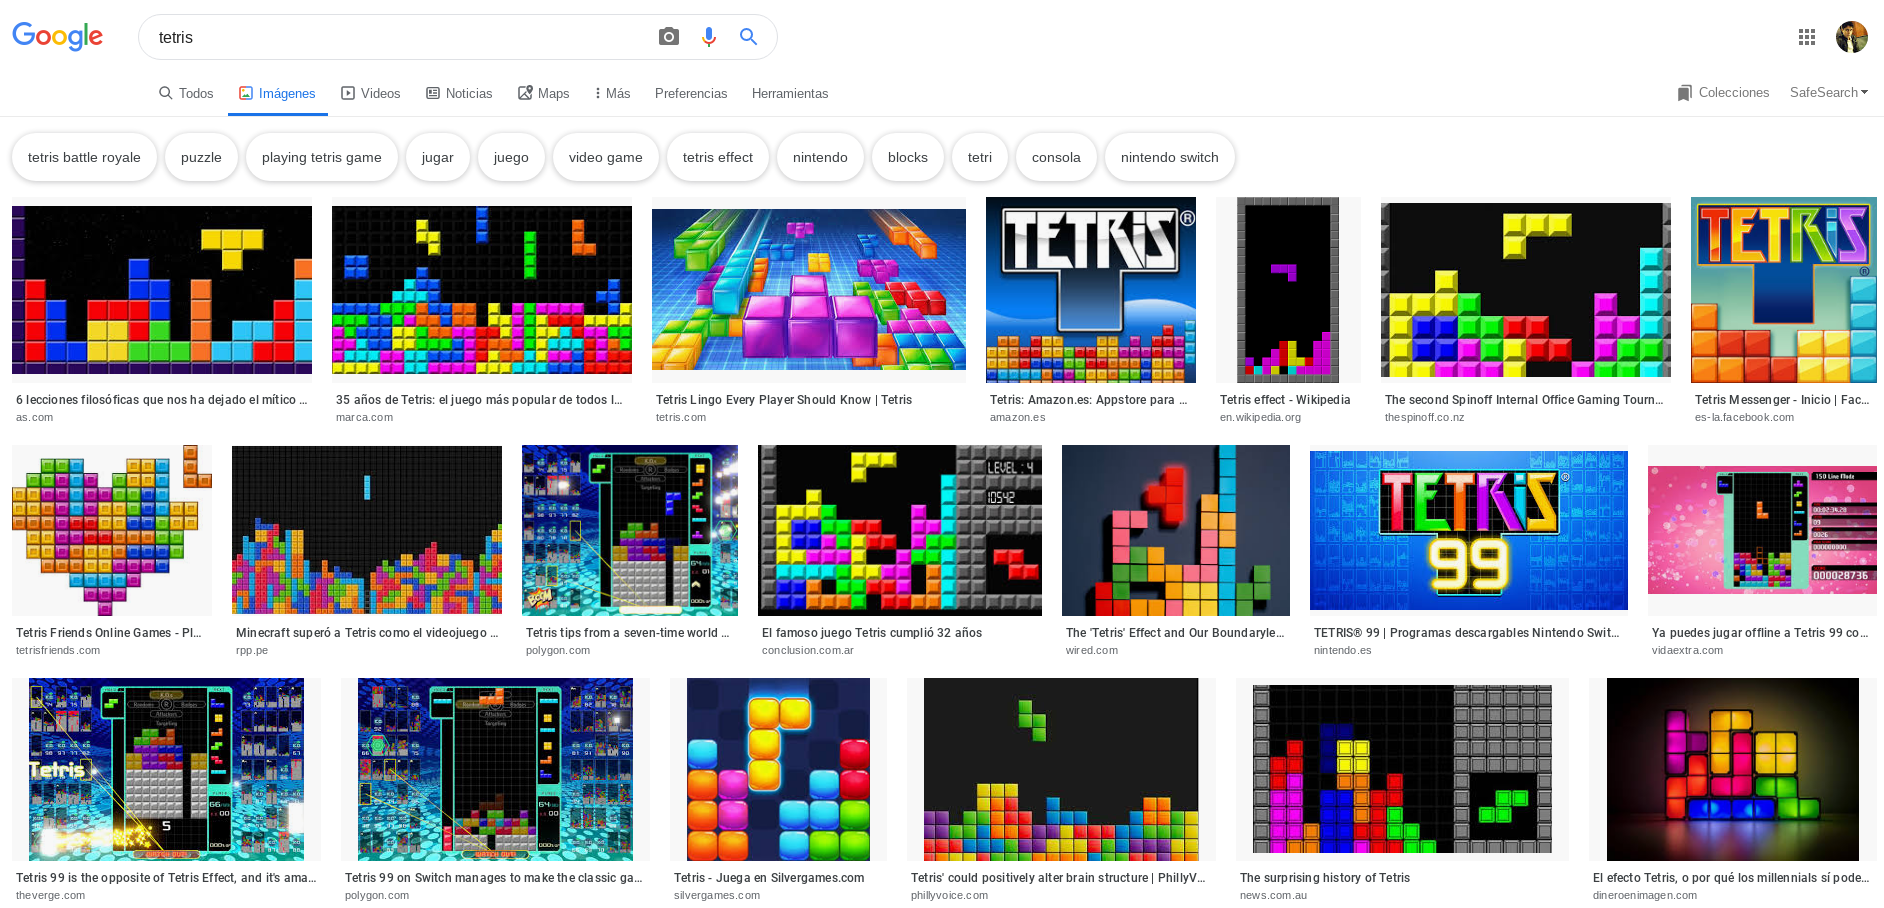
\includegraphics[scale=0.15]{./images/tetris_search.png}
\caption{Búsqueda de imágenes de Tetris en Google.}
\end{figure}

\end{frame} 

\begin{frame}
\frametitle{Tetris en la ciencia}

\begin{columns}
\column{0.5\textwidth}
Tetris es un problema ampliamente estudiado por la comunidad científica en distintas áreas: 

\begin{itemize}

\item Psicología
\item Matemáticas
\item Termodinámica
\item Ciencias de la Computación{\onslide<2->}:
\begin{itemize}

\item ¿Existe una estrategia para jugar en un tiempo indeterminado? 
\item ¿Cuál es la mejor estrategia de juego?
\item \textcolor<3->{red}{¿Existe alguna manera eficiente y automatizada de jugar Tetris?}
\item[] 

\end{itemize}
{\onslide}
\end{itemize}

\column{0.5\textwidth}
\begin{figure}
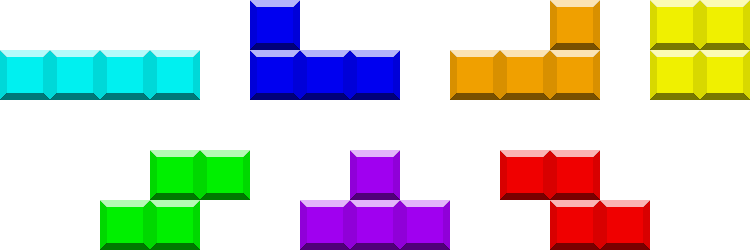
\includegraphics[scale=0.4]{./images/tetrominos.pdf}
\caption{Las piezas de Tetris.}
\end{figure}
\end{columns}


\end{frame}

\input{./tetris.tex}

\begin{frame}
\frametitle{Clasificación de problemas}

Primera clasificación:

\begin{itemize}
\item \textit{Entscheidungsproblem} (El problema de decisión).
\pause
\begin{columns}
\column{0.5\textwidth}
\begin{figure}
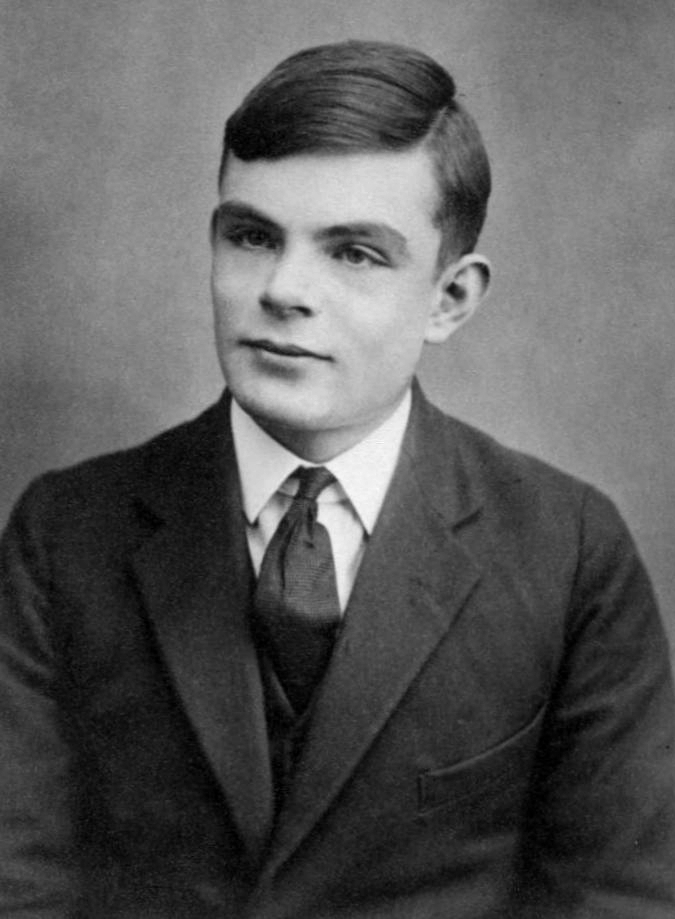
\includegraphics[scale=0.096]{./images/Turing.jpg}
\caption{Alan Turing}
\end{figure}
\column{0.5\textwidth}
\begin{figure}
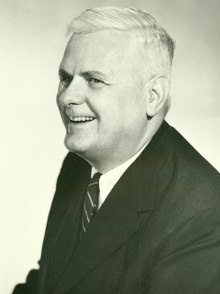
\includegraphics[scale=0.3]{./images/Church.jpg}
\caption{Alonzo Church}
\end{figure}
\end{columns}
\pause
\item Medición de tiempo y espacio en función de la entrada.
\begin{itemize}
\item Juris Hartmanis.
\item Richard Stearns.
\end{itemize}
\end{itemize}
\end{frame}



\begin{frame}
\frametitle{Clasificación de problemas}
Clases de complejidad:
\begin{itemize}
\item El lenguaje $L$ está en \textsl{P} $\Leftrightarrow$ cumple que: 
\begin{itemize}
\item $M$ corre en tiempo polinomial para toda entrada
\item $\forall x \in L, M(x) = TRUE \lor FALSE$.
\end{itemize}
\pause
\item Un lenguaje $L \in $ \textsl{NP} $\rightarrow \exists$ un
  polinomio $p: \mathbb{N} \longrightarrow \mathbb{N}$ y una MT $M$ 
  tal que $\forall x \in \{0,1\}^{*}$, 
  
  \begin{displaymath}
    x \in L \Leftrightarrow \exists u \in \{0,1\}^{p(|x|)},~
    \textrm{tal que} ~ M(x,u) = 1.
  \end{displaymath}
  \pause
\item Se dice que $L'$ es \textsl{NP}-duro si
  $L \leq_{p} L'$ para cada $L \in \textsl{NP} $.
  \pause
\item  Se dice que $L'$ es \textsl{NP}-completo si $L'$ es \textsl{NP}-duro y
  $L' \in \textsl{NP}$.
\end{itemize}

%\begin{itemize}
%\item Ejemplo de \textsl{NP}-completo: \texttt{3-PARTITION}
%\end{itemize}
\end{frame}

\begin{frame}
\frametitle{Tipo de soluciones}

Algoritmo:
\begin{block}{Definición (usada en este trabajo)}
 Un algoritmo es cualquier procedimiento bien
definido que toma algún valor, o conjunto de valores como entrada
(o \textbf{Input}) y produce algún valor, o conjunto de valores como
salida (u \textbf{Output}). Un algoritmo siempre termina.
\end{block}

\pause

Ejemplos: 

\begin{itemize}
\item Suma de los primeros $n \in \mathbb{N}$ ($O(n)$).
\item Mergesort ($O(n\log(n))$).
\item Algoritmo de Dijkstra ($O(|E| + |V|\log(|V|))$).
\end{itemize}

\pause

\begin{itemize}
		\item[$\blacksquare$] Ventaja: Garantía de resultado.
		\item[$\blacksquare$] Desventaja: Tiempo poco realista en problemas $\notin$ \textsl{P}.
\end{itemize}

\end{frame}


\begin{frame}
\frametitle{Algoritmos fuera de la clase \textsl{P}}

\begin{block}{3-SAT}
Dado un conjunto de fórmulas
$\phi = \{x_{1}, x_{2}, x_{3}, ..., x_{n}\}$ con cada $x_{i}$ una fórmula lógica
de la forma $x_{i} = p_{i} \lor q_{i} \lor r_{i} $, con $ p_{i}, q_{i}, r_{i}$,
variables o términos lógicos, se deberá encontrar una
interpretación $\mathcal{I}$ tal que $\mathcal{I}(\phi) = \mathcal{I}(x_{i}) = 1$
$\forall i \in \{1,2,...,n\}$.
\end{block}
\pause
¿Qué pasa si aplicamos un algoritmo para encontrar la solución de un problema como \texttt{3-SAT} $\in$ \textsl{NP}-completo?

\begin{columns}
\column{0.5\textwidth}
\begin{figure}[h]
\scalebox{.4}{% GNUPLOT: LaTeX picture
\setlength{\unitlength}{0.240900pt}
\ifx\plotpoint\undefined\newsavebox{\plotpoint}\fi
\sbox{\plotpoint}{\rule[-0.200pt]{0.400pt}{0.400pt}}%
\begin{picture}(1500,900)(0,0)
\sbox{\plotpoint}{\rule[-0.200pt]{0.400pt}{0.400pt}}%
\put(171.0,131.0){\rule[-0.200pt]{4.818pt}{0.400pt}}
\put(151,131){\makebox(0,0)[r]{$0$}}
\put(1419.0,131.0){\rule[-0.200pt]{4.818pt}{0.400pt}}
\put(171.0,313.0){\rule[-0.200pt]{4.818pt}{0.400pt}}
\put(151,313){\makebox(0,0)[r]{$500$}}
\put(1419.0,313.0){\rule[-0.200pt]{4.818pt}{0.400pt}}
\put(171.0,495.0){\rule[-0.200pt]{4.818pt}{0.400pt}}
\put(151,495){\makebox(0,0)[r]{$1,000$}}
\put(1419.0,495.0){\rule[-0.200pt]{4.818pt}{0.400pt}}
\put(171.0,677.0){\rule[-0.200pt]{4.818pt}{0.400pt}}
\put(151,677){\makebox(0,0)[r]{$1,500$}}
\put(1419.0,677.0){\rule[-0.200pt]{4.818pt}{0.400pt}}
\put(171.0,859.0){\rule[-0.200pt]{4.818pt}{0.400pt}}
\put(151,859){\makebox(0,0)[r]{$2,000$}}
\put(1419.0,859.0){\rule[-0.200pt]{4.818pt}{0.400pt}}
\put(171.0,131.0){\rule[-0.200pt]{0.400pt}{4.818pt}}
\put(171,90){\makebox(0,0){$2$}}
\put(171.0,839.0){\rule[-0.200pt]{0.400pt}{4.818pt}}
\put(488.0,131.0){\rule[-0.200pt]{0.400pt}{4.818pt}}
\put(488,90){\makebox(0,0){$3$}}
\put(488.0,839.0){\rule[-0.200pt]{0.400pt}{4.818pt}}
\put(805.0,131.0){\rule[-0.200pt]{0.400pt}{4.818pt}}
\put(805,90){\makebox(0,0){$4$}}
\put(805.0,839.0){\rule[-0.200pt]{0.400pt}{4.818pt}}
\put(1122.0,131.0){\rule[-0.200pt]{0.400pt}{4.818pt}}
\put(1122,90){\makebox(0,0){$5$}}
\put(1122.0,839.0){\rule[-0.200pt]{0.400pt}{4.818pt}}
\put(1439.0,131.0){\rule[-0.200pt]{0.400pt}{4.818pt}}
\put(1439,90){\makebox(0,0){$6$}}
\put(1439.0,839.0){\rule[-0.200pt]{0.400pt}{4.818pt}}
\put(171.0,131.0){\rule[-0.200pt]{0.400pt}{175.375pt}}
\put(171.0,131.0){\rule[-0.200pt]{305.461pt}{0.400pt}}
\put(1439.0,131.0){\rule[-0.200pt]{0.400pt}{175.375pt}}
\put(171.0,859.0){\rule[-0.200pt]{305.461pt}{0.400pt}}
\put(30,495){\rotatebox{90}{\makebox(0,0){Asignaciones}}
}\put(805,29){\makebox(0,0){Fórmulas}}
\put(488,136){\usebox{\plotpoint}}
\multiput(488.00,136.58)(3.894,0.498){79}{\rule{3.193pt}{0.120pt}}
\multiput(488.00,135.17)(310.373,41.000){2}{\rule{1.596pt}{0.400pt}}
\multiput(805.58,177.00)(0.500,0.514){631}{\rule{0.120pt}{0.511pt}}
\multiput(804.17,177.00)(317.000,324.939){2}{\rule{0.400pt}{0.256pt}}
\put(488,136){\makebox(0,0){$+$}}
\put(805,177){\makebox(0,0){$+$}}
\put(1122,503){\makebox(0,0){$+$}}
\put(1122.0,503.0){\rule[-0.200pt]{0.400pt}{85.760pt}}
\put(171.0,131.0){\rule[-0.200pt]{0.400pt}{175.375pt}}
\put(171.0,131.0){\rule[-0.200pt]{305.461pt}{0.400pt}}
\put(1439.0,131.0){\rule[-0.200pt]{0.400pt}{175.375pt}}
\put(171.0,859.0){\rule[-0.200pt]{305.461pt}{0.400pt}}
\end{picture}
}
\end{figure} 

\column{0.5\textwidth}
\begin{figure}
\scalebox{.4}{\begin{figure}[H]
\centering
\begin{tikzpicture}[level/.style={sibling distance=50mm/#1}]
\node [circle,draw] (z){$\varphi_{1}$}
  child {node [circle,draw] (a) {$\varphi_{2}$}
    child {node [circle,draw] (b) {$\varphi_{3}$}
      child {node (p1) {$\vdots$}
        child {node [circle,draw] (d) {$\varphi_{n}$}}
        child {node [circle,draw] (e) {$\varphi_{n}$}}
      }
      child {node (p2) {$\vdots$}}
    }
    child {node [circle,draw] (g) {$\varphi_{3}$}
      child {node (p3) {$\vdots$}}
      child {node (p4) {$\vdots$}}
    }
  }
  child {node [circle,draw] (j) {$\varphi_{2}$}
    child {node [circle,draw] (k) {$\varphi_{3}$}
      child {node (p5) {$\vdots$}}
      child {node (p6) {$\vdots$}}
    }
  child {node [circle,draw] (l) {$\varphi_{3}$}
    child {node (p7) {$\vdots$}}
    child {node (c){$\vdots$}
      child {node [circle,draw] (o) {$\varphi_{n}$}}
      child {node [circle,draw] (p) {$\varphi_{n}$}
        child [grow=right] {node (q) {$=$} edge from parent[draw=none]
          child [grow=right] {node (q) {$O(2^{n})$} edge from parent[draw=none]
            child [grow=up] {node (r) {$\vdots$} edge from parent[draw=none]
              child [grow=up] {node (s) {$O(2^{3}=8)$} edge from parent[draw=none]
                child [grow=up] {node (t) {$O(2^{2}=4)$} edge from parent[draw=none]
                  child [grow=up] {node (u) {$O(2^{1})=2$} edge from parent[draw=none]}
                }
              }
            }
            child [grow=down] {node (v) {$O\left(\displaystyle\sum_{i = 1}^n 2^n \right)$}edge from parent[draw=none]}
          }
        }
      }
    }
  }
};
\path (a) -- (j) node [midway] {+};
\path (b) -- (g) node [midway] {+};
\path (k) -- (l) node [midway] {+};
\path (k) -- (g) node [midway] {+};
\path (d) -- (e) node [midway] {+};
\path (o) -- (p) node [midway] {+};
\path (o) -- (e) node (x) [midway] {$\cdots$};
\path (q) -- (r) node [midway] {+};
\path (s) -- (r) node [midway] {+};
\path (s) -- (t) node [midway] {+};
\path (s) -- (l) node [midway] {=};
\path (t) -- (u) node [midway] {+};
\path (z) -- (u) node [midway] {=};
\path (j) -- (t) node [midway] {=};
\path (q) -- (v) node [midway] {=};



\path (z) edge node[above=3pt]{$1$} (a);
\path (z) edge node[above=3pt]{$0$} (j);

\path (a) edge node[left]{$1$} (b);
\path (a) edge node[right]{$0$} (g);
\path (j) edge node[left]{$1$} (k);
\path (j) edge node[right]{$0$} (l);

\path (b) edge node[left]{$1$} (p1);
\path (b) edge node[right]{$0$} (p2);
\path (g) edge node[left]{$1$} (p3);
\path (g) edge node[right]{$0$} (p4);
\path (k) edge node[left]{$1$} (p5);
\path (k) edge node[right]{$0$} (p6);
\path (l) edge node[left]{$1$} (p7);
\path (l) edge node[right]{$0$} (c);

\path (p1) edge node[left]{$1$} (d);
\path (p1) edge node[right]{$0$} (e);
\path (c) edge node[left]{$1$} (o);
\path (c) edge node[right]{$0$} (p);

\end{tikzpicture}
\caption{Posibles valores de verdad por cada variable en un árbol binario.} \label{fig:a3sat02}
\end{figure}}
\end{figure}

\end{columns}
\end{frame}

\begin{frame}
\frametitle{Tipo de soluciones}

Heurística:
\begin{block}{Definición}
Las heurísticas, al igual que los algoritmos, también son una secuencia de pasos bien definida con la diferencia de que dada una
entrada $I$, produce una salida $o \in \texttt{OUTPUT}$ con $\texttt{OUTPUT}$ un
conjunto de posibles valores de solución. Durante la ejecución de una heurística, la condición de término es más ambigua.
\end{block}

\pause

Ejemplos: 


\begin{itemize}
\item Heurísticas usadas para optimización de redes neuronales.
\item Búsqueda tabú.
\item Algoritmos (heurísticos) genéticos.
\end{itemize}

\pause

\begin{itemize}
		\item[$\blacksquare$] Ventaja: Reducción significativa en tiempo de respuesta.
		\item[$\blacksquare$] Desventaja: Desempeño pobre en el peor de los casos.
\end{itemize}

\end{frame}

\begin{frame}
\frametitle{Colonia de abejas artificiales}

\begin{columns}

\column{0.5\textwidth}
\begin{itemize}
\item ¿Agentes involucrados?
\pause
\begin{itemize}
\item Abejas exploradoras.
\item Abejas trabajadoras.
\item Abejas observadoras.
\end{itemize}
\pause
\item Comportamiento colectivo.
\pause

\item Recomendaciones basadas en resultados de experimentación del autor Dervis Karaboga.
\end{itemize}

{\onslide<3->}
\column{0.5\textwidth}
\begin{figure}
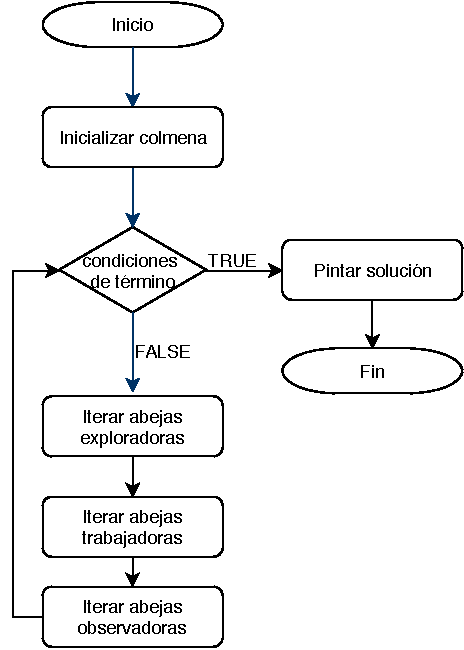
\includegraphics[scale=0.5]{./images/diagrama-flujo.pdf}
\end{figure}
{\onslide}

\end{columns}

\end{frame}

\begin{frame}
\frametitle{Justificación de aplicación de la heurística}

\begin{columns}
\column{0.5\textwidth}
... 

\begin{itemize}

\item Psicología
\item Matemáticas
\item Termodinámica
\item Ciencias de la Computación:
\begin{itemize}

\item ¿Existe una estrategia para jugar en un tiempo indeterminado? 
\item ¿Cuál es la mejor estrategia de juego?
\item \textcolor<1>{red}{¿Existe alguna manera eficiente y automatizada de jugar Tetris?}
{\onslide<2->}
\item \textcolor{red}{¿A qué clase (\textsl{P, NP, NP}-duro o \textsl{NP}-completo) pertenece Tetris?} 
{\onslide}
\end{itemize}

\end{itemize}

\column{0.5\textwidth}
\begin{figure}
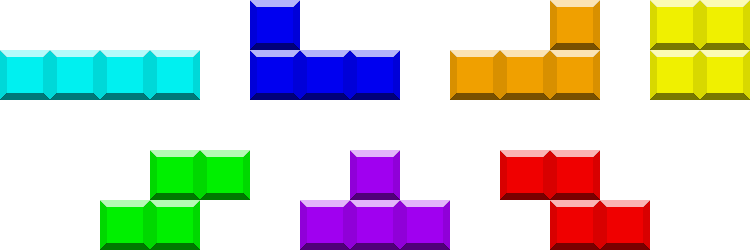
\includegraphics[scale=0.4]{./images/tetrominos.pdf}
\caption{Las piezas de Tetris.}
\end{figure}
\end{columns}

\end{frame}


\begin{frame}
\frametitle{Clasificación de \texttt{TETRIS}}
\pause
\begin{itemize}
\item Formalización del juego:
\begin{itemize}
\pause
\item Tablero: matriz de $n$ por $m$ filas.
\pause
\item Piezas: $P = \langle t, o, \langle i,j \rangle, f \rangle$.
\pause
\item Rotación: $R: \langle P, \theta, B \rangle \mapsto P'$.
\pause
\item Reglas del juego: 
\pause
\begin{itemize}
\item $R(P, 90^{\circ}, B)$.
\item $R(P, -90^{\circ}, B)$.
\item $P' = \langle t, o, \langle i - 1,j \rangle, \texttt{MOVIBLE}\rangle$.
\item $P' = \langle t, o, \langle i + 1,j \rangle, \texttt{MOVIBLE}\rangle$.
\item $P' = \langle t, o, \langle i,j - 1 \rangle, \texttt{MOVIBLE}\rangle$.
\item $P' = \langle t, o, \langle i,j \rangle, \texttt{FIJO}\rangle$.
\end{itemize}
\end{itemize}
\pause
\item \texttt{TETRIS}:
\begin{itemize}

\item \textbf{Input:} Un juego de Tetris de la forma 
$\mathcal{G} = \langle B, P_{1}, P_{2}, ..., P_{p} \rangle$.

\item \textbf{Output:} ¿Existe la secuencia de trayectorias $\Sigma$ tal que 
$\Phi(\mathcal{G}, \Sigma)$ no resulte en una partida perdida?

\end{itemize}
\pause
\item Demostración: ¿Es \texttt{TETRIS} \textsl{NP}? \buonslide[red][1pt]<10->{¿Es \texttt{TETRIS} \textsl{NP}-duro?} {\onslide<11->} $\longrightarrow$ Es \texttt{TETRIS} \textsl{NP}-completo.	
{\onslide}
\end{itemize}
\end{frame}

\begin{frame}
\frametitle{Tecnologías}
\pause
\begin{figure}
\centering

\includegraphics[scale=0.03]{./images/python.png}
\end{figure}

\pause

\begin{center}
\arrowdown 
\end{center}

\begin{figure}
\centering


\includegraphics[scale=0.05]{./images/pygame.png}
\end{figure}

\pause

\begin{columns}

\column{0.5\textwidth}
\begin{figure}
\centering

\includegraphics[scale=0.10]{./images/git.jpeg}
\end{figure}

\pause

\column{0.5\textwidth}
\begin{figure}
\centering
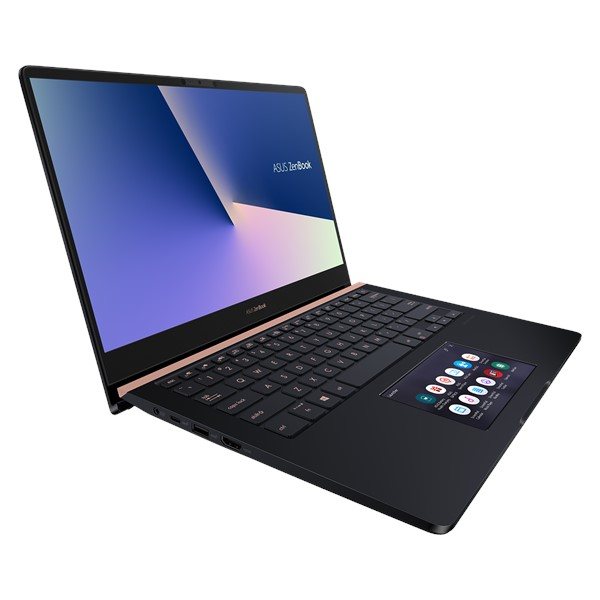
\includegraphics[scale=0.10]{./images/zenbook.jpeg}
\end{figure}

\end{columns}
\end{frame}

\begin{frame}
\frametitle{Diseño de la implementación}
\begin{itemize}
\pause
\item Análisis del sistema.
\pause
\begin{itemize}
\item Mantener modelo apegado a la formalización del juego.
\item Desarrollar la heurística descrita por Dervis Karaboga.
\item Comunicación de la heurística con el juego de Tetris.
\pause
\begin{figure}
\hbox{\hspace{4.5em} \scalebox{.55}{\begin{figure}[H]
\centering
\begin{tikzpicture}
\umlsimpleclass[x=-6, y=1]{\_\_main\_\_.py}
\begin{umlpackage}[x=-6,y=0.7,scale=0.1, name=union]{}
\end{umlpackage}


\begin{umlpackage}[x=0 ,y=0]{test}
\dots
\end{umlpackage}

\begin{umlpackage}[x=0 ,y=0]{abejas-tetris}

\begin{umlpackage}[x=-3 ,y=-3]{abc}
\dots
\end{umlpackage}

\begin{umlpackage}[x=3 ,y=3]{tetris}
\dots
\end{umlpackage}

\umlclass[x=0, y=0]{Abejas\_Tetris}{
$\qquad\quad\dots$
}{
$\qquad\quad\dots$ 
}

\end{umlpackage}
\umlimport[geometry=|-,anchor1=0, anchor2=west, name=import]{abc}{test}
\umlimport[geometry=|-, name=import]{tetris}{test}
\umlimport[geometry=|-,anchor1=north, anchor2=90, name=import]{test}{union}
\end{tikzpicture}
\caption{Estructura básica del sistema.} \label{fig:uml-estructura}
\end{figure}}}
\end{figure}
\end{itemize}
\end{itemize}
\pause
\begin{center}
Orientación a Objetos
\end{center}
\end{frame}


\begin{frame}
\frametitle{Diseño de clases}
\pause
\LARGE
Tetris:
\normalsize

\begin{columns}
\column{0.5\textwidth}
\begin{itemize}
\item Punto.
\item Tipo.
\item Casilla.
\end{itemize}

\column{0.5\textwidth}
\begin{itemize}
\item Pieza.
\item Tablero.
\item Tetris.
\end{itemize}
\end{columns}
\pause

\vspace{10mm}

\LARGE
ABC:
\normalsize
\pause
\begin{columns}
\column{0.5\textwidth}
\begin{itemize}
\item Tipo\_Abeja.
\item Colmena.
\end{itemize}

\column{0.5\textwidth}
\begin{itemize}
\item Abeja:
\pause
\begin{itemize}
\item Exploradoras.
\item Trabajadoras.
\item \textcolor<6->{red}{Observadoras.}
\end{itemize}
\end{itemize}
\end{columns}

\end{frame}



\begin{frame}
\frametitle{Abejas observadoras}
\begin{itemize}
\item ¿Qué hacen exactamente las abejas observadoras en ABC? 
\begin{itemize}
\pause
\item Seleccionan una fuente $i$: 
\begin{displaymath}
  P_{i} = \frac{F(\theta_{i})}{\sum_{k=1}^{n} F(\theta_{k})}.
\end{displaymath}
\pause
\item Buscan una fuente vecina a $i$:
\begin{displaymath}
  \theta_{i}(c+1) = \theta_{i}(c) \pm \phi_{i}(c).
\end{displaymath}
\end{itemize}
\pause
\item ¿Cómo se proyecta una fuente en Tetris?
\pause
R= Para un juego $\langle B_{0}, P_{1}, ..., P_{p} \rangle$, una secuencia de
trayectorias $\Sigma$ es una secuencia $B_{0},\sigma_{1},B_{1},...,\sigma_{p},B_{p}$
tal que para cada $i$, la trayectoria de la pieza $P_{i}$ aplicado al tablero
$B_{i-1}$, genera el tablero $B_{i}$.
\end{itemize}
\end{frame}



\begin{frame}
\frametitle{Abejas observadoras}
\begin{itemize}
\item ¿Cómo se \textit{mueven} las abejas \textit{cerca} de una fuente?
\end{itemize}
\begin{figure}
\scalebox{.55}{\begin{tikzpicture}[
    node distance = 21mm and 7mm,
    box/.style = {draw, minimum size=8mm, inner sep=0pt, outer sep=0pt, anchor=center},
      pin edge = {Straight Barb-, shorten <=1mm,semithick}]
        \node (h2) [box] {Izq};
		\node (h1) [box, left=of h2] {Der};
		\node (h3) [box, right=of h2]    {Gir};
		\node (h4) [box, right=of h3]    {Cae};
		\node (q_dots) [draw=none, right=of h4] {$\cdots$};
		\node (hk) [box, right=of q_dots] {$Mov_{m}$};
		
		\node (h5) [box, below=of h4] {Izq};
		\node (h32) [draw=none, left=of h5] {};
		\node (q_dots_two) [draw=none, right=of h5] {$\cdots$};
		\node (hl) [box, below=of hk] {$Mov_{n}$};
		
		
		\draw[dashed,-Straight Barb, shorten <=1mm, shorten >=1mm]
    (h3.south) edge [bend right]   (h5.north);	
		
		\draw[-Straight Barb, transform canvas={yshift= 0mm}]
    		(h1) edge   (h2);
    	\draw[-Straight Barb, transform canvas={yshift= 0mm}]
    		(h2) edge   (h3);
    	\draw[-Straight Barb, transform canvas={yshift= 0mm}]
    		(h3) edge   (h4);
    	\draw[-Straight Barb, transform canvas={yshift= 0mm}]
    		(h4) edge   (q_dots);    		
    	\draw[-Straight Barb, transform canvas={yshift= 0mm}]
    		(h5) edge   (q_dots_two);
    	\draw[-Straight Barb, transform canvas={yshift= 0mm}]
    		(q_dots_two) edge   (hl);
    	\draw[-Straight Barb, transform canvas={yshift= 0mm}]
    		(q_dots) edge   (hk);
    	\draw [decorate,decoration={brace,amplitude=6pt,raise=5ex}]
  (h1) -- (hk) node[midway,yshift=4em]{$\theta_{i}$};
  
 		 \draw [decorate,decoration={brace,amplitude=7pt,mirror,raise=5ex}]
  (h32) -- (hl) node[midway,yshift=-4em]{$\phi_{i}$};
    \end{tikzpicture}
}
\end{figure}
\end{frame}

\begin{frame}
\frametitle{Funciones de las abejas}
\begin{itemize}
\item Abeja exploradora.
\begin{itemize}
\item \texttt{\_busca\_fuente}: Copia la mejor fuente reportada en la colmena y genera un nuevo tablero $B_{n}$ a partir de una trayectoria $\sigma_{n-1}$. $B_{n}$ es ahora su fuente asociada.
\end{itemize}
\pause

\item Abeja trabajadora.
\begin{itemize}
\item \texttt{\_explotar}: Genera un $\sigma_{n}$ sobre su tablero asociado y lo aplica para obtener un tablero nuevo $B_{n+1}$.
\end{itemize}
\pause

\item Abeja observadora.
\begin{itemize}
\item \texttt{\_observadoras}: 
\begin{enumerate}
 \item Se le asigna una fuente de alguna abeja trabajadora. Todas las abejas observadoras tienen que poseer una fuente asociada.
 \item Corta parcialmente la ultima trayectoria $\sigma$ y la completa hasta encontrar una fuente ``cercana''.
 \item Si la fuente cercana es \textit{mejor} a la fuente original, avisa a la colmena. 
\end{enumerate}
\end{itemize}
\pause
\item Todas las abejas.
\begin{itemize}
\item \texttt{\_nectar}: Función de costo o función \textit{fitness}.
\end{itemize}
\end{itemize}
\end{frame}


\begin{frame}
\frametitle{Función de costo}
\begin{itemize}
\item ¿Cuál es el objetivo de la función de costo?
\pause
\begin{itemize}
\item Primer objetivo: que la heurística elimine $n \geq 10$ filas.
\pause
\item Objetivo principal: eliminar $n \geq 20$ filas.
\end{itemize}
\pause
\item ¿Cómo se logra orientar a la heurística hacia el objetivo? 
\pause
Suponer la siguiente entrada: \texttt{L = \{I, Rg, Lg, Sq, 
I, T, Ls, Rs, I\}}.
\begin{columns}
\column{0.45\textwidth}
\begin{figure}
\scalebox{.40}{\begin{figure}[H]
\centering
% 4 es Sq
% 1 es I
% 2 es L(Lg) inversa y 6 es L(Rg)
% 3 es S(Rs) y Z es 7(Ls)
% 5 es T 
% 1, 6, 2, 4, 1, 5, 7, 3, 1
% I, Rg, Lg, Sq, I, T, Ls, Rs, I
\begin{tikzpicture}[omino/nodes/.style={shape=rectangle, rounded corners, inner sep=+0pt, minimum size=1cm-2\pgflinewidth}]
	\path [omino={at={-2,0}, rotate=0}][tetris=1];
	\path [omino={at={4,0}, rotate=0}][tetris=1];
    \path [omino={at={2,0}, rotate=0}][tetris=4];
	\path [omino={at={1,0}, rotate=0}][tetris=2];	
	\path [omino={at={0,0}, rotate=0}][tetris=6];
	\path [omino={at={5,0}, rotate=0}][tetris=5];
	\path [omino={at={7,1}, rotate=0}][tetris=7];
	\path [omino={at={-2,4}, rotate=0}][tetris=3];
	\path [omino={at={0,3}, rotate=0}][tetris=1];
%    \path [omino/at=0:1] [tetris=2];
%    \path [omino/at=0:2] [tetris=3];
%    \path [omino={at=0:3, rotate=-90, x mirror}][tetris=5];
%    \path [omino={at={5,1}, rotate=-90}][tetris=3];
%    \path [omino={at={5,2}, rotate=-90}][tetris=2];
%    \path [omino={at={4,2}, x mirror}][tetris=5];
%    \path [omino={at={1,3}}][tetris=4];
\end{tikzpicture}
\caption{Una mala función de costo deja muchas casillas atrapadas y cubiertas.} \label{fig:mal-juego}
\end{figure}}
\end{figure}
\pause
\column{0.1\textwidth}
\begin{center}
$\Longrightarrow$
\end{center}
\column{0.45\textwidth}
\begin{figure}
\scalebox{.40}{\begin{figure}[H]
\centering
\begin{tikzpicture}[omino/nodes/.style={shape=rectangle, rounded corners, inner sep=+0pt, minimum size=1cm-2\pgflinewidth}]
	\path [omino={at={-1,-2}, rotate=0}][tetris=1];
	\path [omino={at={3,1}, rotate=90}][tetris=1];
    \path [omino={at={1,-1}, rotate=0}] [tetris=4];
	\path [omino={at={3,0}, rotate=180}][tetris=2];	
	\path [omino={at={0,0}, rotate=180}][tetris=6];
	\path [omino={at={6,-2}, rotate=90}][tetris=5];
	\path [omino={at={4,-1}, rotate=0}][tetris=3];
	\path [omino={at={8,-2}, rotate=0}][tetris=1];
	\path [omino={at={7,-2}, rotate=0}] [tetris=7];	
%    \path [omino/at=0:1] [tetris=2];
%    \path [omino/at=0:2] [tetris=3];
%    \path [omino={at=0:3, rotate=-90, x mirror}][tetris=5];
%    \path [omino={at={5,1}, rotate=-90}][tetris=3];
%    \path [omino={at={5,2}, rotate=-90}][tetris=2];
%    \path [omino={at={4,2}, x mirror}][tetris=5];
%    \path [omino={at={1,3}}][tetris=4];
\end{tikzpicture}
\caption{Una función que pareciera funcionar mejor al trata de cubrir todos los espacios.} \label{fig:medio-juego}
\end{figure}}
\end{figure}
\end{columns}

\item ¿Cómo se sabe que una función de costo funciona acorde a los requerimientos?
\pause
\textcolor{red}{Experimentación}.
\end{itemize}


\end{frame}

\begin{frame}
\frametitle{Filas entre pesos negativos}
\begin{displaymath}
   f = \frac{1 + \texttt{filas-removidas}}{\texttt{horizontalidad} + \texttt{atrapados} + \texttt{cubiertos} + \texttt{altura}} .
\end{displaymath}
\pause 
\begin{columns}
\column{0.45\textwidth}
\begin{figure}
\scalebox{.40}{\begin{figure}[H]
\centering
% 4 es Sq
% 1 es I
% 2 es L(Lg) inversa y 6 es L(Rg)
% 3 es S(Rs) y Z es 7(Ls)
% 5 es T 
% 1, 1, 4, 4, 4, 4
% I, I, Sq, Sq, Sq, Sq
\begin{tikzpicture}[omino/nodes/.style={shape=rectangle, rounded corners, inner sep=+0pt, minimum size=1cm-2\pgflinewidth}]
	\path [omino={at={0,0}, rotate=0}][tetris=2];
	\path [omino={at={4,0}, rotate=0}][tetris=4];
	\path [omino={at={5,2}, rotate=90}][tetris=1];
	\path [omino={at={9,0}, rotate=90}][tetris=1];	
	\path [omino={at={6,1}, rotate=0}][tetris=4];
	\path [omino={at={9,3}, rotate=180}][tetris=5];
\end{tikzpicture}
\caption{De izquierda a derecha las fichas son \texttt{Lg, I1, Sq1, Sq2, I2, T}.} \label{fig:eval-tablero}
\end{figure}}
\end{figure}
\begin{itemize}
\pause
\item $\texttt{filas-removidas} = 0$
\item $\texttt{horizontalidad} = 1$
\item $\texttt{atrapados} = 1$
\item $\texttt{cubiertos} = 7$
\item $\texttt{altura} = 4$ 
\end{itemize}
\begin{displaymath}
    \frac{1 + \texttt{0}}{\texttt{1} + \texttt{1} + \texttt{7} + \texttt{4}} = \frac{1}{13} \approx 0.077.
\end{displaymath}
\pause
\column{0.1\textwidth}
\begin{center}
VS.
\end{center}
\column{0.45\textwidth}
\begin{figure}
\scalebox{.40}{\begin{figure}[H]
\centering
% 4 es Sq
% 1 es I
% 2 es L(Lg) inversa y 6 es L(Rg)
% 3 es S(Rs) y Z es 7(Ls)
% 5 es T 
% 1, 1, 4, 4, 4, 4
% I, I, Sq, Sq, Sq, Sq
\begin{tikzpicture}[omino/nodes/.style={shape=rectangle, rounded corners, inner sep=+0pt, minimum size=1cm-2\pgflinewidth}]
	\path [omino={at={9,2}, rotate=180}][tetris=2];
	\path [omino={at={2,0}, rotate=0}][tetris=4];
	\path [omino={at={7,0}, rotate=90}][tetris=1];
	\path [omino={at={8,1}, rotate=90}][tetris=1];	
	\path [omino={at={0	,0}, rotate=0}][tetris=4];
	\path [omino={at={3,2}, rotate=-90}][tetris=5];
\end{tikzpicture}
\caption{Tablero que toma las piezas de la \cref{fig:eval-tablero} y la función de filas entre pesos negativos.} \label{fig:eval-tablero-dos}
\end{figure}}
\end{figure}
\begin{itemize}
\pause
\item $\texttt{filas-removidas} = 2$
\item $\texttt{horizontalidad} = 1$
\item $\texttt{atrapados} = 0$
\item $\texttt{cubiertos} = 0$
\item $\texttt{altura} = 4$ 
\end{itemize}
\begin{displaymath}
    \frac{1 + (2 \times c)}{1 + 0 + 0 + 1} = \frac{1 + 4}{2} = \frac{5}{2} = 2.5.
\end{displaymath}
\end{columns}

\end{frame}

\begin{frame}
\frametitle{Resultados filas entre pesos negativos}
En una colmena de 100 abejas, los resultados fueron los siguientes:
\begin{figure}
\scalebox{.7}{% GNUPLOT: LaTeX picture
\setlength{\unitlength}{0.240900pt}
\ifx\plotpoint\undefined\newsavebox{\plotpoint}\fi
\sbox{\plotpoint}{\rule[-0.200pt]{0.400pt}{0.400pt}}%
\begin{picture}(1500,900)(0,0)
\sbox{\plotpoint}{\rule[-0.200pt]{0.400pt}{0.400pt}}%
\put(131.0,131.0){\rule[-0.200pt]{4.818pt}{0.400pt}}
\put(111,131){\makebox(0,0)[r]{$0$}}
\put(1419.0,131.0){\rule[-0.200pt]{4.818pt}{0.400pt}}
\put(131.0,313.0){\rule[-0.200pt]{4.818pt}{0.400pt}}
\put(111,313){\makebox(0,0)[r]{$5$}}
\put(1419.0,313.0){\rule[-0.200pt]{4.818pt}{0.400pt}}
\put(131.0,495.0){\rule[-0.200pt]{4.818pt}{0.400pt}}
\put(111,495){\makebox(0,0)[r]{$10$}}
\put(1419.0,495.0){\rule[-0.200pt]{4.818pt}{0.400pt}}
\put(131.0,677.0){\rule[-0.200pt]{4.818pt}{0.400pt}}
\put(111,677){\makebox(0,0)[r]{$15$}}
\put(1419.0,677.0){\rule[-0.200pt]{4.818pt}{0.400pt}}
\put(131.0,859.0){\rule[-0.200pt]{4.818pt}{0.400pt}}
\put(111,859){\makebox(0,0)[r]{$20$}}
\put(1419.0,859.0){\rule[-0.200pt]{4.818pt}{0.400pt}}
\put(131.0,131.0){\rule[-0.200pt]{0.400pt}{4.818pt}}
\put(131,90){\makebox(0,0){$0$}}
\put(131.0,839.0){\rule[-0.200pt]{0.400pt}{4.818pt}}
\put(393.0,131.0){\rule[-0.200pt]{0.400pt}{4.818pt}}
\put(393,90){\makebox(0,0){$200$}}
\put(393.0,839.0){\rule[-0.200pt]{0.400pt}{4.818pt}}
\put(654.0,131.0){\rule[-0.200pt]{0.400pt}{4.818pt}}
\put(654,90){\makebox(0,0){$400$}}
\put(654.0,839.0){\rule[-0.200pt]{0.400pt}{4.818pt}}
\put(916.0,131.0){\rule[-0.200pt]{0.400pt}{4.818pt}}
\put(916,90){\makebox(0,0){$600$}}
\put(916.0,839.0){\rule[-0.200pt]{0.400pt}{4.818pt}}
\put(1177.0,131.0){\rule[-0.200pt]{0.400pt}{4.818pt}}
\put(1177,90){\makebox(0,0){$800$}}
\put(1177.0,839.0){\rule[-0.200pt]{0.400pt}{4.818pt}}
\put(1439.0,131.0){\rule[-0.200pt]{0.400pt}{4.818pt}}
\put(1439,90){\makebox(0,0){$1000$}}
\put(1439.0,839.0){\rule[-0.200pt]{0.400pt}{4.818pt}}
\put(131.0,131.0){\rule[-0.200pt]{0.400pt}{175.375pt}}
\put(131.0,131.0){\rule[-0.200pt]{315.097pt}{0.400pt}}
\put(1439.0,131.0){\rule[-0.200pt]{0.400pt}{175.375pt}}
\put(131.0,859.0){\rule[-0.200pt]{315.097pt}{0.400pt}}
\put(30,495){\rotatebox{-270}{\makebox(0,0){Filas eliminadas}}
}\put(785,29){\makebox(0,0){Semillas probadas}}
\put(1279,818){\makebox(0,0)[r]{Filas entre pesos neg}}
\put(1299.0,818.0){\rule[-0.200pt]{24.090pt}{0.400pt}}
\put(132,313){\usebox{\plotpoint}}
\multiput(132.58,313.00)(0.492,1.530){21}{\rule{0.119pt}{1.300pt}}
\multiput(131.17,313.00)(12.000,33.302){2}{\rule{0.400pt}{0.650pt}}
\multiput(144.00,349.58)(0.809,0.499){143}{\rule{0.747pt}{0.120pt}}
\multiput(144.00,348.17)(116.450,73.000){2}{\rule{0.373pt}{0.400pt}}
\multiput(262.00,422.58)(0.899,0.499){143}{\rule{0.818pt}{0.120pt}}
\multiput(262.00,421.17)(129.303,73.000){2}{\rule{0.409pt}{0.400pt}}
\multiput(393.00,495.58)(1.078,0.500){361}{\rule{0.962pt}{0.120pt}}
\multiput(393.00,494.17)(390.004,182.000){2}{\rule{0.481pt}{0.400pt}}
\multiput(785.00,677.58)(3.008,0.499){215}{\rule{2.500pt}{0.120pt}}
\multiput(785.00,676.17)(648.811,109.000){2}{\rule{1.250pt}{0.400pt}}
\put(131.0,131.0){\rule[-0.200pt]{0.400pt}{175.375pt}}
\put(131.0,131.0){\rule[-0.200pt]{315.097pt}{0.400pt}}
\put(1439.0,131.0){\rule[-0.200pt]{0.400pt}{175.375pt}}
\put(131.0,859.0){\rule[-0.200pt]{315.097pt}{0.400pt}}
\end{picture}
}
\pause
\begin{itemize}
\item Se obtuvieron como mejor solución 18 filas removidas.
\end{itemize}
\end{figure}
\end{frame}


\begin{frame}
\frametitle{\textit{Raining skyline}}
\begin{itemize}
\item Optimización de casillas disponibles. ¿En qué consiste?
\end{itemize}
\begin{columns}
\column{0.45\textwidth}
\begin{figure}
\scalebox{.40}{\begin{figure}[H]
\centering
% 4 es Sq
% 1 es I
% 2 es L(Lg) inversa y 6 es L(Rg)
% 3 es S(Rs) y Z es 7(Ls)
% 5 es T 
% 1, 1, 4, 4, 4, 4
% I, I, Sq, Sq, Sq, Sq
\begin{tikzpicture}[omino/nodes/.style={shape=rectangle, rounded corners, inner sep=+0pt, minimum size=1cm-2\pgflinewidth}]
	
	\path [omino={at={-2,0}, rotate=0}][tetris=0];
	\path [omino={at={-1,0}, rotate=0}][tetris=0];
	\path [omino={at={0,0}, rotate=0}][tetris=0];
	\path [omino={at={1,0}, rotate=0}][tetris=0];
	\path [omino={at={2,0}, rotate=0}][tetris=0];
	\path [omino={at={3,0}, rotate=0}][tetris=0];
	\path [omino={at={4,0}, rotate=0}][tetris=0];
	\path [omino={at={5,0}, rotate=0}][tetris=0];
	\path [omino={at={6,0}, rotate=0}][tetris=0];
	\path [omino={at={7,0}, rotate=0}][tetris=0];
	
	\path [omino={at={-2,1}, rotate=0}][tetris=0];
	\path [omino={at={-1,1}, rotate=0}][tetris=0];
	\path [omino={at={0,1}, rotate=0}][tetris=0];	
	\path [omino={at={1,1}, rotate=0}][tetris=0];
	\path [omino={at={2,1}, rotate=0}][tetris=0];
	\path [omino={at={3,1}, rotate=0}][tetris=0];
	\path [omino={at={4,1}, rotate=0}][tetris=0];
	\path [omino={at={5,1}, rotate=0}][tetris=0];
	\path [omino={at={6,1}, rotate=0}][tetris=0];
	\path [omino={at={7,1}, rotate=0}][tetris=0];

	
	\path [omino={at={-2,2}, rotate=0}][tetris=0];
	\path [omino={at={-1,2}, rotate=0}][tetris=0];
	\path [omino={at={0,2}, rotate=0}][tetris=0];
	\path [omino={at={1,2}, rotate=0}][tetris=0];
	\path [omino={at={2,2}, rotate=0}][tetris=0];
	\path [omino={at={3,2}, rotate=0}][tetris=0];
	\path [omino={at={4,2}, rotate=0}][tetris=0];
	\path [omino={at={5,2}, rotate=0}][tetris=0];
	\path [omino={at={6,2}, rotate=0}][tetris=0];
	\path [omino={at={7,2}, rotate=0}][tetris=0];
	
	\path [omino={at={-2,3}, rotate=0}][tetris=0];
	\path [omino={at={-1,3}, rotate=0}][tetris=0];
	\path [omino={at={0,3}, rotate=0}][tetris=0];
	\path [omino={at={1,3}, rotate=0}][tetris=0];
	\path [omino={at={2,3}, rotate=0}][tetris=0];
	\path [omino={at={3,3}, rotate=0}][tetris=0];
	\path [omino={at={4,3}, rotate=0}][tetris=0];
	\path [omino={at={5,3}, rotate=0}][tetris=0];
	\path [omino={at={6,3}, rotate=0}][tetris=0];
	\path [omino={at={7,3}, rotate=0}][tetris=0];	
	
	\path [omino={at={-2,4}, rotate=0}][tetris=0];
	\path [omino={at={-1,4}, rotate=0}][tetris=0];
	\path [omino={at={0,4}, rotate=0}][tetris=0];
	\path [omino={at={1,4}, rotate=0}][tetris=0];
	\path [omino={at={2,4}, rotate=0}][tetris=0];
	\path [omino={at={3,4}, rotate=0}][tetris=0];
	\path [omino={at={4,4}, rotate=0}][tetris=0];
	\path [omino={at={5,4}, rotate=0}][tetris=0];
	\path [omino={at={6,4}, rotate=0}][tetris=0];
	\path [omino={at={7,4}, rotate=0}][tetris=0];	
	
	\path [omino={at={-2,5}, rotate=0}][tetris=0];
	\path [omino={at={-1,5}, rotate=0}][tetris=0];
	\path [omino={at={0,5}, rotate=0}][tetris=0];
	\path [omino={at={1,5}, rotate=0}][tetris=0];
	\path [omino={at={2,5}, rotate=0}][tetris=0];
	\path [omino={at={3,5}, rotate=0}][tetris=0];
	\path [omino={at={4,5}, rotate=0}][tetris=0];
	\path [omino={at={5,5}, rotate=0}][tetris=0];
	\path [omino={at={6,5}, rotate=0}][tetris=0];
	\path [omino={at={7,5}, rotate=0}][tetris=0];	
	
	\path [omino={at={-2,6}, rotate=0}][tetris=0];
	\path [omino={at={-1,6}, rotate=0}][tetris=0];
	\path [omino={at={0,6}, rotate=0}][tetris=0];
	\path [omino={at={1,6}, rotate=0}][tetris=0];
	\path [omino={at={2,6}, rotate=0}][tetris=0];
	\path [omino={at={3,6}, rotate=0}][tetris=0];
	\path [omino={at={4,6}, rotate=0}][tetris=0];
	\path [omino={at={5,6}, rotate=0}][tetris=0];
	\path [omino={at={6,6}, rotate=0}][tetris=0];
	\path [omino={at={7,6}, rotate=0}][tetris=0];			
	
	\path [omino={at={0,1}, rotate=90}][tetris=7];
	\path [omino={at={2,3}, rotate=90}][tetris=7];
	\path [omino={at={3,0}, rotate=0}][tetris=4];
	\path [omino={at={4,2}, rotate=0}][tetris=4];
	\path [omino={at={7,0}, rotate=90}][tetris=5];	
\end{tikzpicture}
\caption{Tablero aleatorio con cinco piezas de altura cuatro.} \label{fig:tablero-promedio-uno}
\end{figure}}
\end{figure}
\pause
\column{0.1\textwidth}
\begin{center}
$\Longrightarrow$
\end{center}
\column{0.45\textwidth}
\begin{figure}
\scalebox{.40}{\begin{figure}[H]
\centering
% 4 es Sq
% 1 es I
% 2 es L(Lg) inversa y 6 es L(Rg)
% 3 es S(Rs) y Z es 7(Ls)
% 5 es T 
% 1, 1, 4, 4, 4, 4
% I, I, Sq, Sq, Sq, Sq
\begin{tikzpicture}[omino/nodes/.style={shape=rectangle, rounded corners, inner sep=+0pt, minimum size=1cm-2\pgflinewidth}]
	%\path [omino={at={0,0}, rotate=0}][tetris=8];
	%\path [omino={at={1,1}, rotate=0}][tetris=9];
	
	\path [omino={at={-2,0}, rotate=0}][tetris=9];
	\path [omino={at={-1,0}, rotate=0}][tetris=9];
	\path [omino={at={0,0}, rotate=0}][tetris=9];
	\path [omino={at={1,0}, rotate=0}][tetris=9];
	\path [omino={at={2,0}, rotate=0}][tetris=9];
	\path [omino={at={3,0}, rotate=0}][tetris=9];
	\path [omino={at={4,0}, rotate=0}][tetris=9];
	\path [omino={at={5,0}, rotate=0}][tetris=9];
	\path [omino={at={6,0}, rotate=0}][tetris=9];
	\path [omino={at={7,0}, rotate=0}][tetris=9];
	
	\path [omino={at={-2,1}, rotate=0}][tetris=8];
	\path [omino={at={-1,1}, rotate=0}][tetris=9];
	\path [omino={at={0,1}, rotate=0}][tetris=9];	
	\path [omino={at={1,1}, rotate=0}][tetris=9];
	\path [omino={at={2,1}, rotate=0}][tetris=9];
	\path [omino={at={3,1}, rotate=0}][tetris=9];
	\path [omino={at={4,1}, rotate=0}][tetris=9];
	\path [omino={at={5,1}, rotate=0}][tetris=9];
	\path [omino={at={6,1}, rotate=0}][tetris=9];
	\path [omino={at={7,1}, rotate=0}][tetris=8];

	
	\path [omino={at={-2,2}, rotate=0}][tetris=8];
	\path [omino={at={-1,2}, rotate=0}][tetris=8];
	\path [omino={at={0,2}, rotate=0}][tetris=9];
	\path [omino={at={1,2}, rotate=0}][tetris=9];
	\path [omino={at={2,2}, rotate=0}][tetris=9];
	\path [omino={at={3,2}, rotate=0}][tetris=8];
	\path [omino={at={4,2}, rotate=0}][tetris=9];
	\path [omino={at={5,2}, rotate=0}][tetris=9];
	\path [omino={at={6,2}, rotate=0}][tetris=8];
	\path [omino={at={7,2}, rotate=0}][tetris=8];
	
	\path [omino={at={-2,3}, rotate=0}][tetris=8];
	\path [omino={at={-1,3}, rotate=0}][tetris=8];
	\path [omino={at={0,3}, rotate=0}][tetris=8];
	\path [omino={at={1,3}, rotate=0}][tetris=9];
	\path [omino={at={2,3}, rotate=0}][tetris=9];
	\path [omino={at={3,3}, rotate=0}][tetris=8];
	\path [omino={at={4,3}, rotate=0}][tetris=9];
	\path [omino={at={5,3}, rotate=0}][tetris=9];
	\path [omino={at={6,3}, rotate=0}][tetris=8];
	\path [omino={at={7,3}, rotate=0}][tetris=8];	
	
	\path [omino={at={-2,4}, rotate=0}][tetris=8];
	\path [omino={at={-1,4}, rotate=0}][tetris=8];
	\path [omino={at={0,4}, rotate=0}][tetris=8];
	\path [omino={at={1,4}, rotate=0}][tetris=8];
	\path [omino={at={2,4}, rotate=0}][tetris=8];
	\path [omino={at={3,4}, rotate=0}][tetris=8];
	\path [omino={at={4,4}, rotate=0}][tetris=8];
	\path [omino={at={5,4}, rotate=0}][tetris=8];
	\path [omino={at={6,4}, rotate=0}][tetris=8];
	\path [omino={at={7,4}, rotate=0}][tetris=8];	
	
	\path [omino={at={-2,5}, rotate=0}][tetris=8];
	\path [omino={at={-1,5}, rotate=0}][tetris=8];
	\path [omino={at={0,5}, rotate=0}][tetris=8];
	\path [omino={at={1,5}, rotate=0}][tetris=8];
	\path [omino={at={2,5}, rotate=0}][tetris=8];
	\path [omino={at={3,5}, rotate=0}][tetris=8];
	\path [omino={at={4,5}, rotate=0}][tetris=8];
	\path [omino={at={5,5}, rotate=0}][tetris=8];
	\path [omino={at={6,5}, rotate=0}][tetris=8];
	\path [omino={at={7,5}, rotate=0}][tetris=8];	
	
	\path [omino={at={-2,6}, rotate=0}][tetris=8];
	\path [omino={at={-1,6}, rotate=0}][tetris=8];
	\path [omino={at={0,6}, rotate=0}][tetris=8];
	\path [omino={at={1,6}, rotate=0}][tetris=8];
	\path [omino={at={2,6}, rotate=0}][tetris=8];
	\path [omino={at={3,6}, rotate=0}][tetris=8];
	\path [omino={at={4,6}, rotate=0}][tetris=8];
	\path [omino={at={5,6}, rotate=0}][tetris=8];
	\path [omino={at={6,6}, rotate=0}][tetris=8];
	\path [omino={at={7,6}, rotate=0}][tetris=8];		
	
		
\end{tikzpicture}
\caption{Ejemplo de cuál es el raining skyline (en rosado) del tablero en la \cref{fig:tablero-promedio-uno}.} \label{fig:raining skyline}
\end{figure}}
\end{figure}
\end{columns}
\pause
\vspace{10mm}
\begin{displaymath}
  rs = \sum_{i=1,j=1}^{ancho, alto} j \enskip | \enskip (i,j) \in C_{sup}.
\end{displaymath} 
\hspace{10mm}
\begin{displaymath}
  f(T) = \frac{n - rs}{n}.
\end{displaymath} 
\end{frame}

\begin{frame}
\frametitle{Resultados de \textit{Raining skyline} sin ponderar}
\begin{figure}
\scalebox{.7}{% GNUPLOT: LaTeX picture
\setlength{\unitlength}{0.240900pt}
\ifx\plotpoint\undefined\newsavebox{\plotpoint}\fi
\sbox{\plotpoint}{\rule[-0.200pt]{0.400pt}{0.400pt}}%
\begin{picture}(1500,900)(0,0)
\sbox{\plotpoint}{\rule[-0.200pt]{0.400pt}{0.400pt}}%
\put(111.0,252.0){\rule[-0.200pt]{4.818pt}{0.400pt}}
\put(91,252){\makebox(0,0)[r]{$0$}}
\put(1419.0,252.0){\rule[-0.200pt]{4.818pt}{0.400pt}}
\put(111.0,859.0){\rule[-0.200pt]{4.818pt}{0.400pt}}
\put(91,859){\makebox(0,0)[r]{$5$}}
\put(1419.0,859.0){\rule[-0.200pt]{4.818pt}{0.400pt}}
\put(111.0,131.0){\rule[-0.200pt]{0.400pt}{4.818pt}}
\put(111,90){\makebox(0,0){$0$}}
\put(111.0,839.0){\rule[-0.200pt]{0.400pt}{4.818pt}}
\put(377.0,131.0){\rule[-0.200pt]{0.400pt}{4.818pt}}
\put(377,90){\makebox(0,0){$1000$}}
\put(377.0,839.0){\rule[-0.200pt]{0.400pt}{4.818pt}}
\put(642.0,131.0){\rule[-0.200pt]{0.400pt}{4.818pt}}
\put(642,90){\makebox(0,0){$2000$}}
\put(642.0,839.0){\rule[-0.200pt]{0.400pt}{4.818pt}}
\put(908.0,131.0){\rule[-0.200pt]{0.400pt}{4.818pt}}
\put(908,90){\makebox(0,0){$3000$}}
\put(908.0,839.0){\rule[-0.200pt]{0.400pt}{4.818pt}}
\put(1173.0,131.0){\rule[-0.200pt]{0.400pt}{4.818pt}}
\put(1173,90){\makebox(0,0){$4000$}}
\put(1173.0,839.0){\rule[-0.200pt]{0.400pt}{4.818pt}}
\put(1439.0,131.0){\rule[-0.200pt]{0.400pt}{4.818pt}}
\put(1439,90){\makebox(0,0){$5000$}}
\put(1439.0,839.0){\rule[-0.200pt]{0.400pt}{4.818pt}}
\put(111.0,131.0){\rule[-0.200pt]{0.400pt}{175.375pt}}
\put(111.0,131.0){\rule[-0.200pt]{319.915pt}{0.400pt}}
\put(1439.0,131.0){\rule[-0.200pt]{0.400pt}{175.375pt}}
\put(111.0,859.0){\rule[-0.200pt]{319.915pt}{0.400pt}}
\put(30,495){\rotatebox{-270}{\makebox(0,0){Filas eliminadas}}
}\put(775,29){\makebox(0,0){Semillas probadas}}
\put(111,616){\usebox{\plotpoint}}
\put(110.67,495){\rule{0.400pt}{29.149pt}}
\multiput(110.17,555.50)(1.000,-60.500){2}{\rule{0.400pt}{14.574pt}}
\put(112.17,252){\rule{0.400pt}{48.700pt}}
\multiput(111.17,393.92)(2.000,-141.921){2}{\rule{0.400pt}{24.350pt}}
\multiput(128.00,252.58)(1.188,0.500){483}{\rule{1.050pt}{0.120pt}}
\multiput(128.00,251.17)(574.821,243.000){2}{\rule{0.525pt}{0.400pt}}
\multiput(705.00,495.58)(0.687,0.500){483}{\rule{0.650pt}{0.120pt}}
\multiput(705.00,494.17)(332.651,243.000){2}{\rule{0.325pt}{0.400pt}}
\put(114.0,252.0){\rule[-0.200pt]{3.373pt}{0.400pt}}
\put(111,616){\makebox(0,0){$+$}}
\put(112,495){\makebox(0,0){$+$}}
\put(114,252){\makebox(0,0){$+$}}
\put(123,252){\makebox(0,0){$+$}}
\put(128,252){\makebox(0,0){$+$}}
\put(705,495){\makebox(0,0){$+$}}
\put(1039,738){\makebox(0,0){$+$}}
\put(1439,738){\makebox(0,0){$+$}}
\put(1039.0,738.0){\rule[-0.200pt]{96.360pt}{0.400pt}}
\put(111.0,131.0){\rule[-0.200pt]{0.400pt}{175.375pt}}
\put(111.0,131.0){\rule[-0.200pt]{319.915pt}{0.400pt}}
\put(1439.0,131.0){\rule[-0.200pt]{0.400pt}{175.375pt}}
\put(111.0,859.0){\rule[-0.200pt]{319.915pt}{0.400pt}}
\end{picture}
}
\end{figure}
\pause
\begin{itemize}
\item ¿Por qué los resultados no son los esperados?
\item ¿Por qué puede decrecer el número de filas eliminadas en una ``mejor'' semilla?
\end{itemize}
\end{frame}

\begin{frame}
\frametitle{Ponderación de \textit{Raining skyline}}
\begin{itemize}
\item[1]
\end{itemize}
\begin{displaymath}
  rs = \sum_{i=1,j=1}^{ancho, alto} j \enskip | \enskip j > b \enskip \land \enskip (i,b) \in C_{sup} 
  \end{displaymath} 

  \begin{displaymath}
    f(T) = \frac{rs}{\sum\limits_{i=1}^{alto} (ancho \times i)}.
\end{displaymath} 
\pause
\begin{itemize}
\item[2]
\end{itemize}
 \begin{displaymath}
    f(T) = \left(\frac{rs}{\sum\limits_{i=1}^{alto} (ancho \times i)}\right) \times (1 + fe).
\end{displaymath} 
\end{frame}

\begin{frame}
\frametitle{Resultados de \textit{Raining skyline} ponderada}
En una colmena de 100 abejas, los resultados fueron los siguientes:
\begin{figure}
\scalebox{.85}{% GNUPLOT: LaTeX picture
\setlength{\unitlength}{0.240900pt}
\ifx\plotpoint\undefined\newsavebox{\plotpoint}\fi
\sbox{\plotpoint}{\rule[-0.200pt]{0.400pt}{0.400pt}}%
\begin{picture}(1500,900)(0,0)
\sbox{\plotpoint}{\rule[-0.200pt]{0.400pt}{0.400pt}}%
\put(131.0,170.0){\rule[-0.200pt]{4.818pt}{0.400pt}}
\put(111,170){\makebox(0,0)[r]{$0$}}
\put(1419.0,170.0){\rule[-0.200pt]{4.818pt}{0.400pt}}
\put(131.0,269.0){\rule[-0.200pt]{4.818pt}{0.400pt}}
\put(111,269){\makebox(0,0)[r]{$5$}}
\put(1419.0,269.0){\rule[-0.200pt]{4.818pt}{0.400pt}}
\put(131.0,367.0){\rule[-0.200pt]{4.818pt}{0.400pt}}
\put(111,367){\makebox(0,0)[r]{$10$}}
\put(1419.0,367.0){\rule[-0.200pt]{4.818pt}{0.400pt}}
\put(131.0,465.0){\rule[-0.200pt]{4.818pt}{0.400pt}}
\put(111,465){\makebox(0,0)[r]{$15$}}
\put(1419.0,465.0){\rule[-0.200pt]{4.818pt}{0.400pt}}
\put(131.0,564.0){\rule[-0.200pt]{4.818pt}{0.400pt}}
\put(111,564){\makebox(0,0)[r]{$20$}}
\put(1419.0,564.0){\rule[-0.200pt]{4.818pt}{0.400pt}}
\put(131.0,662.0){\rule[-0.200pt]{4.818pt}{0.400pt}}
\put(111,662){\makebox(0,0)[r]{$25$}}
\put(1419.0,662.0){\rule[-0.200pt]{4.818pt}{0.400pt}}
\put(131.0,761.0){\rule[-0.200pt]{4.818pt}{0.400pt}}
\put(111,761){\makebox(0,0)[r]{$30$}}
\put(1419.0,761.0){\rule[-0.200pt]{4.818pt}{0.400pt}}
\put(131.0,859.0){\rule[-0.200pt]{4.818pt}{0.400pt}}
\put(111,859){\makebox(0,0)[r]{$35$}}
\put(1419.0,859.0){\rule[-0.200pt]{4.818pt}{0.400pt}}
\put(131.0,131.0){\rule[-0.200pt]{0.400pt}{4.818pt}}
\put(131,90){\makebox(0,0){$0$}}
\put(131.0,839.0){\rule[-0.200pt]{0.400pt}{4.818pt}}
\put(393.0,131.0){\rule[-0.200pt]{0.400pt}{4.818pt}}
\put(393,90){\makebox(0,0){$1000$}}
\put(393.0,839.0){\rule[-0.200pt]{0.400pt}{4.818pt}}
\put(654.0,131.0){\rule[-0.200pt]{0.400pt}{4.818pt}}
\put(654,90){\makebox(0,0){$2000$}}
\put(654.0,839.0){\rule[-0.200pt]{0.400pt}{4.818pt}}
\put(916.0,131.0){\rule[-0.200pt]{0.400pt}{4.818pt}}
\put(916,90){\makebox(0,0){$3000$}}
\put(916.0,839.0){\rule[-0.200pt]{0.400pt}{4.818pt}}
\put(1177.0,131.0){\rule[-0.200pt]{0.400pt}{4.818pt}}
\put(1177,90){\makebox(0,0){$4000$}}
\put(1177.0,839.0){\rule[-0.200pt]{0.400pt}{4.818pt}}
\put(1439.0,131.0){\rule[-0.200pt]{0.400pt}{4.818pt}}
\put(1439,90){\makebox(0,0){$5000$}}
\put(1439.0,839.0){\rule[-0.200pt]{0.400pt}{4.818pt}}
\put(131.0,131.0){\rule[-0.200pt]{0.400pt}{175.375pt}}
\put(131.0,131.0){\rule[-0.200pt]{315.097pt}{0.400pt}}
\put(1439.0,131.0){\rule[-0.200pt]{0.400pt}{175.375pt}}
\put(131.0,859.0){\rule[-0.200pt]{315.097pt}{0.400pt}}
\put(785,525){\makebox(0,0)[l]{Objetivo}}
\put(131,564){\line(1,0){1308}}
\put(30,495){\rotatebox{-270}{\makebox(0,0){Filas eliminadas}}
}\put(785,29){\makebox(0,0){Semillas probadas}}
\put(1279,818){\makebox(0,0)[r]{Función raining-skyline}}
\put(1299.0,818.0){\rule[-0.200pt]{24.090pt}{0.400pt}}
\put(131,229){\usebox{\plotpoint}}
\put(130.67,210){\rule{0.400pt}{4.577pt}}
\multiput(130.17,219.50)(1.000,-9.500){2}{\rule{0.400pt}{2.289pt}}
\put(132.17,170){\rule{0.400pt}{8.100pt}}
\multiput(131.17,193.19)(2.000,-23.188){2}{\rule{0.400pt}{4.050pt}}
\multiput(148.00,170.58)(7.158,0.498){77}{\rule{5.780pt}{0.120pt}}
\multiput(148.00,169.17)(556.003,40.000){2}{\rule{2.890pt}{0.400pt}}
\multiput(716.00,210.58)(4.251,0.498){75}{\rule{3.474pt}{0.120pt}}
\multiput(716.00,209.17)(321.789,39.000){2}{\rule{1.737pt}{0.400pt}}
\put(134.0,170.0){\rule[-0.200pt]{3.373pt}{0.400pt}}
\put(1045.0,249.0){\rule[-0.200pt]{94.915pt}{0.400pt}}
\sbox{\plotpoint}{\rule[-0.500pt]{1.000pt}{1.000pt}}%
\sbox{\plotpoint}{\rule[-0.200pt]{0.400pt}{0.400pt}}%
\put(1279,777){\makebox(0,0)[r]{Función raining-skyline ponderada}}
\sbox{\plotpoint}{\rule[-0.500pt]{1.000pt}{1.000pt}}%
\multiput(1299,777)(20.756,0.000){5}{\usebox{\plotpoint}}
\put(1399,777){\usebox{\plotpoint}}
\put(131,269){\usebox{\plotpoint}}
\multiput(131,269)(0.352,-20.753){3}{\usebox{\plotpoint}}
\put(135.26,210.00){\usebox{\plotpoint}}
\multiput(143,210)(2.574,-20.595){2}{\usebox{\plotpoint}}
\multiput(148,170)(20.322,4.222){28}{\usebox{\plotpoint}}
\multiput(716,288)(19.537,7.007){17}{\usebox{\plotpoint}}
\multiput(1045,406)(20.527,3.074){19}{\usebox{\plotpoint}}
\put(1439,465){\usebox{\plotpoint}}
\put(131,269){\makebox(0,0){$\circ$}}
\put(132,210){\makebox(0,0){$\circ$}}
\put(134,210){\makebox(0,0){$\circ$}}
\put(143,210){\makebox(0,0){$\circ$}}
\put(148,170){\makebox(0,0){$\circ$}}
\put(716,288){\makebox(0,0){$\circ$}}
\put(1045,406){\makebox(0,0){$\circ$}}
\put(1439,465){\makebox(0,0){$\circ$}}
\put(1349,777){\makebox(0,0){$\circ$}}
\sbox{\plotpoint}{\rule[-0.400pt]{0.800pt}{0.800pt}}%
\sbox{\plotpoint}{\rule[-0.200pt]{0.400pt}{0.400pt}}%
\put(1279,736){\makebox(0,0)[r]{Función raining-skyline ponderada por filas eliminadas}}
\sbox{\plotpoint}{\rule[-0.400pt]{0.800pt}{0.800pt}}%
\put(1299.0,736.0){\rule[-0.400pt]{24.090pt}{0.800pt}}
\put(131,308){\usebox{\plotpoint}}
\put(129.84,308){\rule{0.800pt}{14.213pt}}
\multiput(129.34,308.00)(1.000,29.500){2}{\rule{0.800pt}{7.107pt}}
\put(131.34,367){\rule{0.800pt}{9.395pt}}
\multiput(130.34,367.00)(2.000,19.500){2}{\rule{0.800pt}{4.698pt}}
\multiput(135.40,406.00)(0.516,2.441){11}{\rule{0.124pt}{3.756pt}}
\multiput(132.34,406.00)(9.000,32.205){2}{\rule{0.800pt}{1.878pt}}
\multiput(144.38,446.00)(0.560,12.850){3}{\rule{0.135pt}{12.840pt}}
\multiput(141.34,446.00)(5.000,52.350){2}{\rule{0.800pt}{6.420pt}}
\multiput(148.00,526.41)(4.865,0.502){111}{\rule{7.902pt}{0.121pt}}
\multiput(148.00,523.34)(551.600,59.000){2}{\rule{3.951pt}{0.800pt}}
\multiput(716.00,585.41)(9.022,0.506){31}{\rule{14.053pt}{0.122pt}}
\multiput(716.00,582.34)(299.833,19.000){2}{\rule{7.026pt}{0.800pt}}
\multiput(1045.00,604.41)(10.242,0.505){33}{\rule{15.960pt}{0.122pt}}
\multiput(1045.00,601.34)(360.874,20.000){2}{\rule{7.980pt}{0.800pt}}
\put(131,308){\makebox(0,0){$\ast$}}
\put(132,367){\makebox(0,0){$\ast$}}
\put(134,406){\makebox(0,0){$\ast$}}
\put(143,446){\makebox(0,0){$\ast$}}
\put(148,525){\makebox(0,0){$\ast$}}
\put(716,584){\makebox(0,0){$\ast$}}
\put(1045,603){\makebox(0,0){$\ast$}}
\put(1439,623){\makebox(0,0){$\ast$}}
\put(1349,736){\makebox(0,0){$\ast$}}
\sbox{\plotpoint}{\rule[-0.200pt]{0.400pt}{0.400pt}}%
\put(131.0,131.0){\rule[-0.200pt]{0.400pt}{175.375pt}}
\put(131.0,131.0){\rule[-0.200pt]{315.097pt}{0.400pt}}
\put(1439.0,131.0){\rule[-0.200pt]{0.400pt}{175.375pt}}
\put(131.0,859.0){\rule[-0.200pt]{315.097pt}{0.400pt}}
\end{picture}
}
\end{figure}
\end{frame}

\begin{frame}
\frametitle{Observaciones adicionales}
\begin{itemize}
\pause
\item Tamaño de la colmena se mantuvo en 100 abejas.
\pause
\item Cada función fue probada con al menos 10,000 semillas pseudoaleatorias. 
\pause
\item Se consiguieron muestras de números mayores al objetivo (71 filas eliminadas).
\pause 
\item Los resultados de ambas funciones arrojan muestras muy similares.
\begin{figure}
\scalebox{.5}{% GNUPLOT: LaTeX picture
\setlength{\unitlength}{0.240900pt}
\ifx\plotpoint\undefined\newsavebox{\plotpoint}\fi
\sbox{\plotpoint}{\rule[-0.200pt]{0.400pt}{0.400pt}}%
\begin{picture}(1500,900)(0,0)
\sbox{\plotpoint}{\rule[-0.200pt]{0.400pt}{0.400pt}}%
\put(131.0,131.0){\rule[-0.200pt]{4.818pt}{0.400pt}}
\put(111,131){\makebox(0,0)[r]{$0$}}
\put(1419.0,131.0){\rule[-0.200pt]{4.818pt}{0.400pt}}
\put(131.0,235.0){\rule[-0.200pt]{4.818pt}{0.400pt}}
\put(111,235){\makebox(0,0)[r]{$5$}}
\put(1419.0,235.0){\rule[-0.200pt]{4.818pt}{0.400pt}}
\put(131.0,339.0){\rule[-0.200pt]{4.818pt}{0.400pt}}
\put(111,339){\makebox(0,0)[r]{$10$}}
\put(1419.0,339.0){\rule[-0.200pt]{4.818pt}{0.400pt}}
\put(131.0,443.0){\rule[-0.200pt]{4.818pt}{0.400pt}}
\put(111,443){\makebox(0,0)[r]{$15$}}
\put(1419.0,443.0){\rule[-0.200pt]{4.818pt}{0.400pt}}
\put(131.0,547.0){\rule[-0.200pt]{4.818pt}{0.400pt}}
\put(111,547){\makebox(0,0)[r]{$20$}}
\put(1419.0,547.0){\rule[-0.200pt]{4.818pt}{0.400pt}}
\put(131.0,651.0){\rule[-0.200pt]{4.818pt}{0.400pt}}
\put(111,651){\makebox(0,0)[r]{$25$}}
\put(1419.0,651.0){\rule[-0.200pt]{4.818pt}{0.400pt}}
\put(131.0,755.0){\rule[-0.200pt]{4.818pt}{0.400pt}}
\put(111,755){\makebox(0,0)[r]{$30$}}
\put(1419.0,755.0){\rule[-0.200pt]{4.818pt}{0.400pt}}
\put(131.0,859.0){\rule[-0.200pt]{4.818pt}{0.400pt}}
\put(111,859){\makebox(0,0)[r]{$35$}}
\put(1419.0,859.0){\rule[-0.200pt]{4.818pt}{0.400pt}}
\put(131.0,131.0){\rule[-0.200pt]{0.400pt}{4.818pt}}
\put(131,90){\makebox(0,0){$0$}}
\put(131.0,839.0){\rule[-0.200pt]{0.400pt}{4.818pt}}
\put(393.0,131.0){\rule[-0.200pt]{0.400pt}{4.818pt}}
\put(393,90){\makebox(0,0){$200$}}
\put(393.0,839.0){\rule[-0.200pt]{0.400pt}{4.818pt}}
\put(654.0,131.0){\rule[-0.200pt]{0.400pt}{4.818pt}}
\put(654,90){\makebox(0,0){$400$}}
\put(654.0,839.0){\rule[-0.200pt]{0.400pt}{4.818pt}}
\put(916.0,131.0){\rule[-0.200pt]{0.400pt}{4.818pt}}
\put(916,90){\makebox(0,0){$600$}}
\put(916.0,839.0){\rule[-0.200pt]{0.400pt}{4.818pt}}
\put(1177.0,131.0){\rule[-0.200pt]{0.400pt}{4.818pt}}
\put(1177,90){\makebox(0,0){$800$}}
\put(1177.0,839.0){\rule[-0.200pt]{0.400pt}{4.818pt}}
\put(1439.0,131.0){\rule[-0.200pt]{0.400pt}{4.818pt}}
\put(1439,90){\makebox(0,0){$1000$}}
\put(1439.0,839.0){\rule[-0.200pt]{0.400pt}{4.818pt}}
\put(131.0,131.0){\rule[-0.200pt]{0.400pt}{175.375pt}}
\put(131.0,131.0){\rule[-0.200pt]{315.097pt}{0.400pt}}
\put(1439.0,131.0){\rule[-0.200pt]{0.400pt}{175.375pt}}
\put(131.0,859.0){\rule[-0.200pt]{315.097pt}{0.400pt}}
\put(30,495){\rotatebox{90}{\makebox(0,0){Filas eliminadas}}
}\put(785,29){\makebox(0,0){Número de pruebas}}
\put(1279,818){\makebox(0,0)[r]{Función raining-skyline}}
\put(1299.0,818.0){\rule[-0.200pt]{24.090pt}{0.400pt}}
\put(131,235){\usebox{\plotpoint}}
\multiput(131.00,235.58)(0.524,0.500){621}{\rule{0.519pt}{0.120pt}}
\multiput(131.00,234.17)(325.922,312.000){2}{\rule{0.260pt}{0.400pt}}
\multiput(785.00,547.58)(1.976,0.499){163}{\rule{1.676pt}{0.120pt}}
\multiput(785.00,546.17)(323.522,83.000){2}{\rule{0.838pt}{0.400pt}}
\multiput(1112.00,630.58)(3.921,0.498){81}{\rule{3.214pt}{0.120pt}}
\multiput(1112.00,629.17)(320.329,42.000){2}{\rule{1.607pt}{0.400pt}}
\put(458.0,547.0){\rule[-0.200pt]{78.774pt}{0.400pt}}
\sbox{\plotpoint}{\rule[-0.600pt]{1.200pt}{1.200pt}}%
\sbox{\plotpoint}{\rule[-0.200pt]{0.400pt}{0.400pt}}%
\put(1279,777){\makebox(0,0)[r]{Función de pesos pos/neg}}
\sbox{\plotpoint}{\rule[-0.600pt]{1.200pt}{1.200pt}}%
\put(1299.0,777.0){\rule[-0.600pt]{24.090pt}{1.200pt}}
\put(131,256){\usebox{\plotpoint}}
\multiput(131.00,258.24)(0.984,0.500){322}{\rule{2.664pt}{0.120pt}}
\multiput(131.00,253.51)(321.471,166.000){2}{\rule{1.332pt}{1.200pt}}
\multiput(458.00,424.24)(0.873,0.500){364}{\rule{2.398pt}{0.120pt}}
\multiput(458.00,419.51)(322.022,187.000){2}{\rule{1.199pt}{1.200pt}}
\multiput(1112.00,611.24)(1.574,0.500){198}{\rule{4.073pt}{0.120pt}}
\multiput(1112.00,606.51)(318.546,104.000){2}{\rule{2.037pt}{1.200pt}}
\put(131,256){\makebox(0,0){$\blacksquare$}}
\put(458,422){\makebox(0,0){$\blacksquare$}}
\put(785,609){\makebox(0,0){$\blacksquare$}}
\put(1112,609){\makebox(0,0){$\blacksquare$}}
\put(1439,713){\makebox(0,0){$\blacksquare$}}
\put(1349,777){\makebox(0,0){$\blacksquare$}}
\put(785.0,609.0){\rule[-0.600pt]{78.774pt}{1.200pt}}
\sbox{\plotpoint}{\rule[-0.200pt]{0.400pt}{0.400pt}}%
\put(131.0,131.0){\rule[-0.200pt]{0.400pt}{175.375pt}}
\put(131.0,131.0){\rule[-0.200pt]{315.097pt}{0.400pt}}
\put(1439.0,131.0){\rule[-0.200pt]{0.400pt}{175.375pt}}
\put(131.0,859.0){\rule[-0.200pt]{315.097pt}{0.400pt}}
\end{picture}
}
\end{figure}
\end{itemize}
\end{frame}

\input{./experimentacion.tex}

\begin{frame}
\frametitle{Conclusiones}
\begin{itemize}
\pause
\item La meta propuesta fue alcanzada exitosamente.
\vspace{10mm}
\pause
\item El comportamiento de la heurística aplicada a Tetris particularmente parece responder positivamente.
\vspace{10mm}
\pause
\item Los resultados obtenidos superan las expectativas.
\end{itemize}
\end{frame}

\begin{frame}
\frametitle{Conclusiones}
\begin{itemize}
\item Sin importar que el problema de Tetris sea un problema \textsl{NP}-completo, existen métodos prácticos que pueden encontrar soluciones de buena calidad.
\vspace{10mm}
\pause
\item La heurística ABC es un buen método de resolución de problemas ya  
que la función de costo de la que depende sus resultados es independiente al 
comportamiento del colectivo en la colmena.
\end{itemize}
\end{frame}

\begin{frame}
\centering
Ejecución del código.
\end{frame}

\end{document}
